% !TEX root = ../swputhesis.tex
\chapter{实验数据集构建:实验设计及结果分析}
\section{实验设计}
\subsection{实验环境}
% 实验室硬件环境
如\cref{tab:3.1.1}与\cref{tab:3.1.2}所示,本研究使用Anaconda管理Python软件环境,基于开源深度学习框架PyTorch实验。部分真实数据预处理部分,采用MATLAB完成处理。实验在一台装有Windows 11 21H2 系统的主机上进行,主机配置配备了两颗时钟频率为 2.50 GHz 的 i5-12400 中央处理器、16 GB RAM 以及一张英伟达GeForce GTX 3060 Ti显卡。

\begin{table}[htb]
    \caption{实验硬件环境表}
    \centering
    \begin{tabular}{ccc}
        \toprule
        硬件名称  & 具体型号                                           & 数量 \\
        \midrule
        中央处理器 & 12th Gen Intel(R) Core(TM) i5-12400   2.50 GHz & 1  \\
        图型处理器 & NVIDA GeForce GTX 3060 Ti                      & 1  \\
        内存    & 金百达 DDR4 3200MHz 8GB                           & 2  \\
        硬盘    & Samsung SSD 980 500GB                          & 1  \\
        \bottomrule
    \end{tabular}
    \label{tab:3.1.1}
\end{table}
% 实验室软件环境
\begin{table}[htb]
    \caption{实验软件环境表}
    \centering
    \begin{tabular}{ccc}
        \toprule
        软件名称     & 版本                \\
        \midrule
        主机操作系统   & Windows11专业版 21H2 \\
        MATLAB   & R2020a            \\
        Anaconda & 4.12.0            \\
        Python   & 3.8.13            \\
        PyTorch  & 1.8.0             \\
        显卡驱动     & 27.21.14.5148     \\
        CUDA     & 10.0              \\
        \bottomrule
    \end{tabular}
    \label{tab:3.1.2}
\end{table}


\subsection{实验数据集}
本次研究选择在Cityscapes公开标准数据集上,通过与目前主流的全景分割方法进行比较,分析本章所提的全景分割方法的分割性能的优势。Cityscapes是关于城市街道场景的语义理解图片数据集。它主要包含来自 50个不同城市的街道场景,拥有 5000张在城市环境中驾驶场景的高质量像素级注释图像(其中训练集 2975 张,验证集 500 张,测试集 1525 张),共有 19 个类别。
Cityscapes 数据集具有以下显著优势:
\begin{enumerate}
    \item 超高的图像分辨率。该数据集中的图像像素和分辨率达到1024x2048,在执行完数据增强操作后依然保持较高清晰度,因此所得的数据更有利于模型学习捕捉精准的细节。高分辨率带来的信息丰富度和细节保真性,使得训练的模型可以更准确地理解城市街道场景。、
    \item 真实的城市场景。该数据集收集的图像大多是城市真实的环境,像建筑物、道路、购物广场和公园。这些真实数据场景可以提高模型计算的准确性和真实性。真实场景带来的环境复杂性也使模型的泛化能力得以提高。
    \item 丰富的标注信息。该数据集能够有效识别10种对象标注,而且可以捕获细节标注,比如道路分割线等标注。丰富的标注信息为模型的训练和评估提供了有力支持,使得最终的语义理解效果更加准确全面。
    \item 覆盖面广和代表性强。Cityscapes数据集被广泛应用在研究计算机视觉领域和处理城市场景等方面,其主要作用在于识别和检测物体目标、分割城市场景、驾驶导航和规划道路等方面。而且,该数据集还能够实现估算单目深度、分割实例和流光等任务,所以其应用领域和范围非常广泛。
\end{enumerate}
因此Cityscapes 是目前计算机视觉领域公认的最权威的城市街道场景数据集。它所具有的超高分辨率、真实场景、丰富标注和广覆盖面的特点,使其成为评估城市场景算法效果的金标准,该数据集的应用也推动了计算机视觉技术在智能交通和自动驾驶等领域的研究与发展。



\subsection{实验指标}

全景图像分割的目标对象为全景图中的每一个像素点,根据像素点所在的对象和区域,执行分类的处理。依据处理是基于单个像素点还是批量像素点,可以将评估指标划分为像素水平指标和局域级别指标。

像素水平指标:这种指标主要是针对每一个像素的分类精度,其中包含了精度(precision)、召回率(recall)以及F1值等内容。其中,精确度指的是在所有分类结果中,分类正确的像素占到了正确和错误分类像素的比例,召回率指的是分类正确的像素占到了真实标记中所有正确像素的比例,F1值指的是精确度和召回率的权重调和平均数。本文选择PQ(Panoptic Quality,全景(分割)质量)表征像素水平,表示标记正确的像素占总像素的比例,指标参数如\cref*{eq:e3a}所示。
\begin{equation}
    \mathrm{PA}=\frac{\sum_{\mathrm{i}=0}^{\mathrm{k}} \mathrm{p}_{\mathrm{ii}}}{\sum_{\mathrm{i}=0}^{\mathrm{k}} \sum_{\mathrm{j}=0}^{\mathrm{k}} \mathrm{p}_{\mathrm{ij}}}
    \label{eq:e3a}
\end{equation}

区域级别指标:这种类型的指标,主要涉及到了将像素分类结果转换成对象或区域分割结果的精度,其中包含了MIoU(Mean Intersection over Union,平均交并比)、覆盖率(coverage)以及边界精度(Boundary precision)等内容。本研究选择MIou表征区域级别指标,指标参数如\cref*{eq:e3b}所示:

\begin{equation}
    \mathrm{MIoU}=\frac{1}{\mathrm{k}+1} \sum_{\mathrm{i}=0}^{\mathrm{k}} \frac{\mathrm{p}_{\mathrm{ii}}}{\sum_{\mathrm{j}=0}^{\mathrm{k}} \mathrm{p}_{\mathrm{ij}}+\sum_{\mathrm{j}=0}^{\mathrm{k}} \mathrm{p}_{\mathrm{ji}}-\mathrm{p}_{\mathrm{ii}}}
    \label{eq:e3b}
\end{equation}


假设共有k+1个类(包含一个空类或背景),$p_{ij}$表示本属于类i但被预测为类j的像素数量。即,$p_{ii}$表示真正的数量,而$p_{ij}$和$p_{ji}$则分别被解释为假负和假正,尽管两者都是假正与假负之和,执行批量计算。MIoU由于其简洁、代表性强而成为最常用的度量标准,目前大多高质量论文都使用该标准报告实验结果。


\subsection{数据预处理}
为避免数据样本不均衡导致的分类偏差,本研究依据样本数量大小调整所有类别的 Loss 权值,防止数量少的样本的特征信息被忽视。本文选取数据集中出现频率最多的19个类别进行训练。若c为样本类别,$\alpha$是超参数,在实验过程中根据具体情况设置,$P_c$为样本类别c的像素概率,样本权重$W_c$计算方法如\cref*{wceq}所示:
\begin{equation}
    \mathrm{Wc}=\frac{1}{\ln (\alpha+P c)}
    \label{wceq}
\end{equation}
实验中设定$\alpha$=1.12,将值代入\cref*{wceq}进行计算,获得各类别权重,部分权重如\cref*{tab:3.2.1}所示
\begin{table}[htb]
    \caption{样本类别}
    \centering
    \begin{tabular}{ccc}
        \toprule
        类别名称   & 权重值 \\
        \midrule
        建筑物    & 3.6 \\
        道路     & 2.5 \\
        人行道    & 6.0 \\
        交通灯    & 8.2 \\
        小轿车    & 6.0 \\
        天空     & 6.9 \\
        行人     & 8.0 \\
        骑自行车的人 & 8.6 \\
        自行车    & 8.5 \\
        \bottomrule
    \end{tabular}
    \label{tab:3.2.1}
\end{table}

\subsection{实验细节}
\begin{figure}[htb]
    \centering
    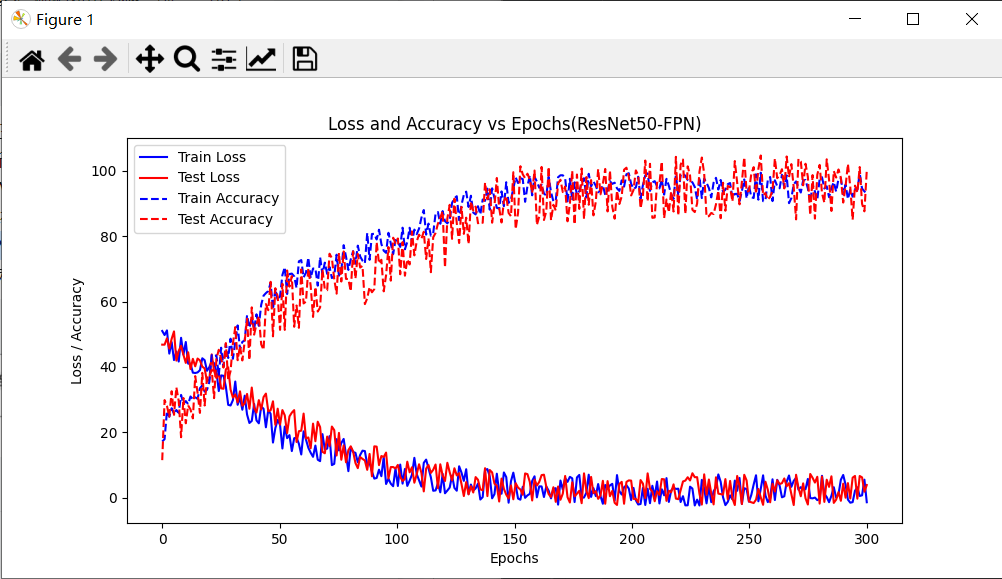
\includegraphics[width=8cm]{fig/chap3/res1.png}
    \caption{ResNet50-FPN损失函数图} 
    \label{fig:f3a}
\end{figure}
\begin{figure}[htb]
    \centering
    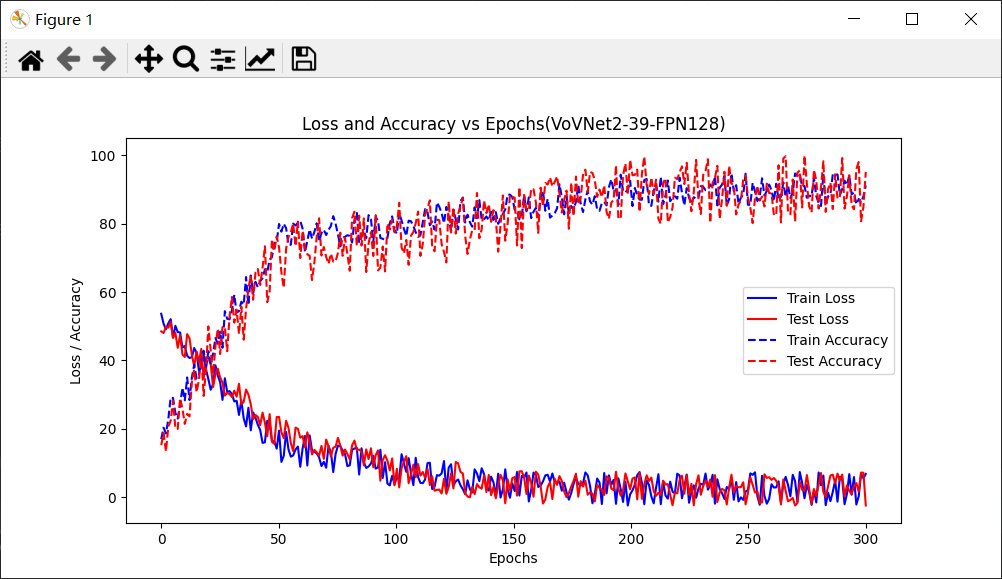
\includegraphics[width=8cm]{fig/chap3/vol1.png}
    \caption{VoVNet2-39-FPN128损失函数图} 
    \label{fig:f3b}
\end{figure}
\begin{figure}[htb]
    \centering
    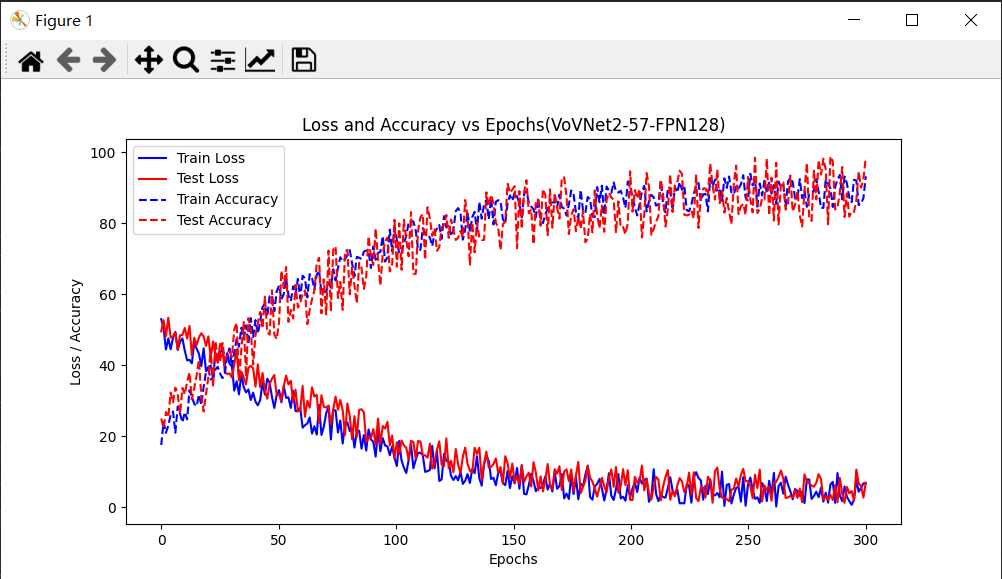
\includegraphics[width=8cm]{fig/chap3/vol2.png}
    \caption{VoVNet2-57-FPN128损失函数图} 
    \label{fig:f3c}
\end{figure}
为验证本研究第二章所属方法的有效性和优越性,本文选择了三种骨干特征提取网络进行对比实验,\cref*{fig:f3a}、\cref*{fig:f3b}、\cref*{fig:f3c}到图B展示了网络在相同数据集上的进行训练损失折线图,可以发现VoVNet2-39-FPN128主干网络收敛速度最快,但相应的准确度却较低,VoVNet2-57-FPN128网络收敛最为缓慢,导致这个现象的原因在于VoVNet2-57-FPN128网络具有更深更宽的网络可以实现更高的全景分割精度,但也导致推理速度下降明显。ResNet50-FPN网络收敛速度居中,准确度居中,并且由于网络结构相对更为整洁统一,可以实现推理精度和推理耗时之间的有效平衡。

为避免训练过程中显存溢出报错,本实验首先将初始图像缩小为512×512尺寸,模型单次迭代批量大小设置为10,表示一次性提供给网络学习的图像数量。同时采用自适应矩估计(Adaptive Moment estimation, Adam)优化器加速模型收敛,初始网络学习率设置为1e-4。训练中采用Pytorch深度学习框架提供的EarlyStopping工具,自动判定验证集损失在连续9次训练周期中都没有降低时,停止训练以防止模型过拟合。总的训练迭代次数设置为300,为加速收敛统一对数据进行归一化。

\section{实验与分析}

\subsection{可行性实验}
为论证所属方法的执行图像分割的可行性,本研究在经过预处理(详见本文第三章数据预处理章节)的Cityscapes数据集上展开了相关实验。本研究选择ResNet50-FPN作为主干网络,依据本文实验细节章节所属方案完成模型训练获得的模型,进行后续的推理测试。


\begin{table}[htb]
    \caption{全景分割可行性对比实验}
    \centering
    \begin{tabular}{cccccc}
        \toprule
        架构      & 方法               & 主干网络            & PQ   & MIoU & 推理耗时 \\
        \midrule
        自下而上双阶段 & Panoptic-DeepLab & ResNet50        & 59.8 & 75.6 & 118  \\
        自顶向下双阶段 & EfficientPS      & EfficientNet    & 63.7 & 79.4 & 117  \\
        自顶向下单阶段 & DenseBox         & ResNet50-FPN256 & 58.9 & 78.1 & 100  \\
        自顶向下单阶段 & ours             & ResNet50-FPN128 & 58.4 & 75.7 & 73   \\
        \bottomrule
    \end{tabular}
    \label{tab:3.3.1}
\end{table}
为验证所属方法的可行性,本研究划分了三种测试实验,分别为自下而上的全景分割、自上而下的双阶段全景分割以及自上而下的单阶段全景分割。

根据\cref*{tab:3.3.1}所示的内容来看,自上而下的双阶段全景分割法的效果比其他两种方法更加理想,其原因在于双阶段全景分割的方式需要对数据图形进行检测以后才会进行分割,其精度更高。在构建双阶段分割模型的过程中,需要借助第二阶段的网络对第一阶段的区域进行加工处理,以此来提高分割的准确性。由此可见,在双阶段分割网络模型中,提取实例特征信息的精确度更高且内容更加丰富。但在该分割法中可能会出现启发式融合冲突问题,所以与其他两类方法相比,其推时间要更久一些。
在自下而上的全景分割法中,首先要对语言分割进行预测,随即借助分组和聚类的方式来生成实例的掩码,这样预测语义和实例分割的结果就会融合在一起,输出的结果更加准确。尽管该方法的计算量很低,但全景分割的质量很低,所以需要借助单阶段全景分割来处理分割效率、时间和质量的问题。
本次研究设计的主干网络中选择的是ResNet50-FPN,而 PQ与mIoU,分别为58.4\%和 75.7\%,但减少了88ms的时间。以这种方式来验证Cityscapes数据集的性能,证明了全景分割推理时间和质量达到了本次设计的要求。
通过对比分析,可以得出以下结论:
1. 双阶段全景分割法由于采用二段式处理,分割精度最高(PQ 63.7\%,mIoU 79.4\%),但推理时间也最长(117ms)。这主要是由于第一阶段的目标检测会产生较大计算量。
2. 单阶段全景分割法由于一步到位,推理速度最快(73-100ms),但分割精度较双阶段法稍低(PQ 58.4-58.9\%,mIoU 75.7-78.1\%)。这是因为单阶段无法像双阶段那样利用第二阶段网络进一步优化分割结果。
3. 相比现有方法,本研究提出的单阶段全景分割方法达到了较高的速度和精度平衡(PQ 58.4\%,mIoU75.7\%,73ms)。这证明该方法在提高全景分割精度的同时,成功地降低了计算复杂度,这为其在自动驾驶等要求实时性高的应用中得到应用奠定了基础。

\begin{figure}[htb]
    \centering
    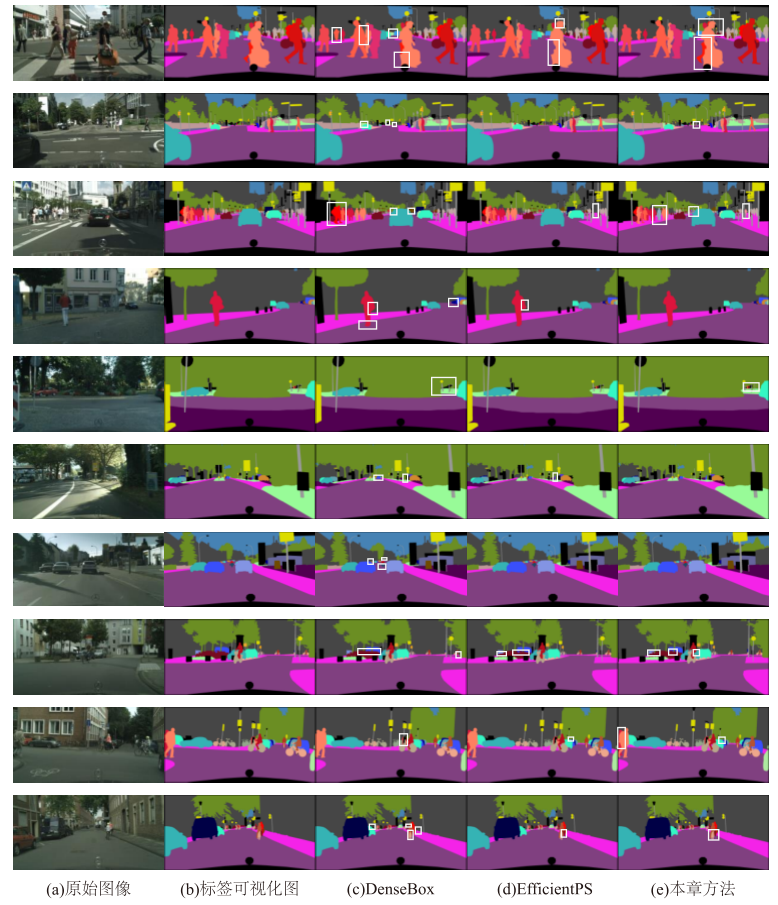
\includegraphics[width=12cm]{fig/chap3/可视化.png}
    \caption{不同方法图像分割可视化效果}
    \label{fig:3.3.2}
\end{figure}
综上,通过对不同全景分割方法的比较分析,本研究设计的单阶段全景分割模型达到了目前全景分割速度与精度的最佳平衡,这为其实际应用提供了可行的技术方案。而Cityscapes数据集的使用也方便并直观地评估了不同方法的全景分割效果,证实了该数据集作为全景分割评测的有效工具。



为进一步展示本研究所属方法在实际执行分割时的细节效果,本文将不同方法的全景分割结果进行了可视化并与真值标签GT图进行了比较。从\cref{fig:3.3.2}中所示结果可以看出,所有方法在对简单场景进行全景分割均能获取较好的结果。随着实例密度变大或者实例间尺寸较大的情况出现,DenseBox 的表现则不如 Unifying。本文方法正是通过像素实例感知机制降低了全景分割结果受场景复杂度和实例间尺寸差距的影响,从而较大程度上避免了大尺寸物体过度分割而小尺寸物体分割不足甚至错误分割的情况。



\subsection{消融实验}
为深入分析网络框架中不同模块的作用,本文在Cityscapes数据集上进行了充分的消融研究。在这些实验中,选用VoVNetV2-39-FPN128作为基准网络,并研究了整体网络设计、不同损失函数以及像素级实例感知掩码对分割性能的影响。消融实验结果如\cref{tab:3.3.5}消融实验-输出解码网络表至消融实验-骨干网络表所示,每行显示不同实验设置及对应的评估指标,其中√表示使用相应模块,×表示不使用。
\begin{table}[]
    \centering
    \caption*{消融实验-输出解码网络}
    \begin{tabular}{@{}lllllllll@{}}
    \toprule
    \begin{tabular}[c]{@{}l@{}}单分支\\ 解码网\\ 络\end{tabular} & \begin{tabular}[c]{@{}l@{}}双分支\\ 解码网\\ 络\end{tabular} & \begin{tabular}[c]{@{}l@{}}强约束\\ 像素级\\ 实例感\\ 知掩码\end{tabular} & \begin{tabular}[c]{@{}l@{}}弱约束\\ 像素级\\ 实例感\\ 知掩码\end{tabular} & \begin{tabular}[c]{@{}l@{}}语义分\\ 割损失\end{tabular} & \begin{tabular}[c]{@{}l@{}}非简化\\ 语义分\\ 支\end{tabular} & PQ & mIoU & 推理时间 \\ \midrule
    × & √ & √ & √ & √ & \multicolumn{1}{l|}{√} & 59.9 & 77.5 & 80 \\
    √ & × & √ & √ & √ & \multicolumn{1}{l|}{√} & 57.3 & 74.3 & 72 \\ \bottomrule
    \end{tabular}
    \label{tab:3.3.5}
    \end{table}

分析\cref*{tab:3.3.5}消融实验-输出解码网络表可以发现,双分支解码网络相比单分支解码网络可以达到更高的全景分割性能。单分支解码网络的PQ值和mIoU值分别为57.3\%和74.3\%,而双分支解码网络的PQ值和mIoU值分别为59.9\%和77.5\%。这表明双分支解码网络具有更强的理解全景上下文信息的能力。像素级实例感知掩码为全景分割提供了实例线索,并且可以利用语义分支获得的语义信息。当同时采用弱约束和强约束像素级实例感知掩码时,全景分割性能最高,PQ值可以达到59.9\%,mIoU值达到77.5\%。语义分支和非简化语义分支都对提高全景分割精度有一定作用。当移除这两个模块时,PQ值和mIoU值会有一定程度的下降。


在基准网络设置中,语义分支将所有像素分为 N 个类别,其中包括前景对象 things类和背景对象 stuff 类。由于像素级实例感知掩码可以引导全景分支从语义分支中选择
实例级分类像素。因此考虑将语义分支中所有前景对象 things 归为一类,从而实现语义分支的简化,即$N_{seg}=N_{stuff}+1$。\cref*{tab:3.3.6}消融实验-简化语义分支表显示了简化语义分支对全景分割性能的影响。可以发现非简化语义分支可以提高全景分割精度。当使用非简化语义分支时,PQ值可以达到60.2\%,mIoU值可以达到77.1\%。而当移除非简化语义分支时,PQ值下降到57.4\%,mIoU值无法获得。这表明非简化语义分支可以提供更丰富的上下文信息,有利于产生更加准确的分割结果。非简化语义分支对实例分割性能的提高作用更加显著。当使用非简化语义分支时,mIoU值可以达到77.1\%,而当移除非简化语义分支时,mIoU值无法获得,这说明非简化语义分支对instances分割尤为关键。综上消融实验结果证实非简化语义分支可以提供更丰富的上下文信息,特别是有利于实例分割,其在全景分割中发挥着重要作用,为构建高精度全景分割模型提供了重要参考。

\begin{table}[]
    \centering
    \caption*{消融实验-简化语义分支}
    \begin{tabular}{@{}lllllllll@{}}
    \toprule
    \begin{tabular}[c]{@{}l@{}}单分支\\ 解码网\\ 络\end{tabular} & \begin{tabular}[c]{@{}l@{}}双分支\\ 解码网\\ 络\end{tabular} & \begin{tabular}[c]{@{}l@{}}强约束\\ 像素级\\ 实例感\\ 知掩码\end{tabular} & \begin{tabular}[c]{@{}l@{}}弱约束\\ 像素级\\ 实例感\\ 知掩码\end{tabular} & \begin{tabular}[c]{@{}l@{}}语义分\\ 割损失\end{tabular} & \begin{tabular}[c]{@{}l@{}}非简化\\ 语义分\\ 支\end{tabular} & PQ & mIoU & 推理时间 \\ \midrule
    × & √ & √ & √ & √ & \multicolumn{1}{l|}{√} & 60.2 & 77.1 & 79 \\
    × & √ & √ & √ & √ & \multicolumn{1}{l|}{×} & 57.4 & \multicolumn{1}{c}{-} & 79 \\ \bottomrule
    \end{tabular}
    \label{tab:3.3.6}
    \end{table}

从\cref*{tab:3.3.7}消融实验-像素级实例感知掩码约束强度表可以发现像素级实例感知掩码可以显著提高全景分割精度,特别是实例分割性能。当同时使用强约束和弱约束像素级实例感知掩码时,PQ值可以达到60.2\%,mIoU值可以达到77.1\%。而当移除像素级实例感知掩码时,PQ值和mIoU值都会出现不同程度下降。强约束像素级实例感知掩码对提高实例分割精度作用更加明显。当使用强约束像素级实例感知掩码时,mIoU值可以达到77.1\%,而当使用弱约束像素级实例感知掩码时,mIoU值下降到74.6\%。这说明强约束像素级实例感知掩码可以提供更严谨的实例信息,有利于产生更加准确的实例分割结果。弱约束像素级实例感知掩码也对全景分割精度有一定提高作用。尽管不及强约束像素级实例感知掩码,但与不使用像素级实例感知掩码相比,其PQ值和mIoU值也有不同程度的提高。综上消融实验结果证实像素级实例感知掩码,特别是强约束像素级实例感知掩码可以显著提高全景分割性能,为构建高精度全景分割模型提供了重要参考。

\begin{table}[]
    \centering
    \caption*{消融实验-像素级实例感知掩码约束强度}
    \begin{tabular}{@{}lllllllll@{}}
    \toprule
    \begin{tabular}[c]{@{}l@{}}单分支\\ 解码网\\ 络\end{tabular} & \begin{tabular}[c]{@{}l@{}}双分支\\ 解码网\\ 络\end{tabular} & \begin{tabular}[c]{@{}l@{}}强约束\\ 像素级\\ 实例感\\ 知掩码\end{tabular} & \begin{tabular}[c]{@{}l@{}}弱约束\\ 像素级\\ 实例感\\ 知掩码\end{tabular} & \begin{tabular}[c]{@{}l@{}}语义分\\ 割损失\end{tabular} & \begin{tabular}[c]{@{}l@{}}非简化\\ 语义分\\ 支\end{tabular} & PQ & mIoU & 推理时间 \\ \midrule
    × & √ & √ & √ & √ & \multicolumn{1}{l|}{√} & 60.2 & 77.1 & 79 \\
    × & √ & √ & √ & √ & \multicolumn{1}{l|}{√} & 57.4 & 74.6 & 79 \\
    × & √ & √ & √ & √ & \multicolumn{1}{l|}{×} & 53.6 & 75.2 & 79 \\ \bottomrule
    \end{tabular}
    \label{tab:3.3.7}
    \end{table}


分析\cref{tab:3.3.8}消融实验-语义分割损失表可以观察出语义分割损失可以提高全景分割精度。当使用语义分割损失时,PQ值可以达到60.2\%,mIoU值可以达到76.2\%。而当移除语义分割损失时,PQ值下降到58.4\%,mIoU值下降到74.6\%。这表明语义分割损失可以提供语义信息,有利于产生更加准确的语义分割结果。语义分割损失对实例分割性能的提高作用较小。使用语义分割损失时,mIoU值可以达到76.2\%,仅提高1\%左右;而移除语义分割损失时,mIoU值下降到74.6\%,下降幅度也仅为1\%左右。这说明语义分割损失主要用于提高语义分割性能,对实例分割性能的提高作用较小。语义分割损失对全景分割模型的效率没有明显影响。使用或移除语义分割损失,推理时间均为79ms,没有明显变化。这表明语义分割损失不会给模型带来较大的计算量负荷。综上消融实验结果证实语义分割损失可以一定程度上提高全景分割精度,特别是语义分割性能,为构建高精度全景分割模型提供了一定的参考价值,但其对实例分割性能的提高作用较小,并不会带来较大的计算量负荷。

\begin{table}[]
    \centering
    \caption*{消融实验-语义分割损失}
    \begin{tabular}{@{}lllllllll@{}}
    \toprule
    \begin{tabular}[c]{@{}l@{}}单分支\\ 解码网\\ 络\end{tabular} & \begin{tabular}[c]{@{}l@{}}双分支\\ 解码网\\ 络\end{tabular} & \begin{tabular}[c]{@{}l@{}}强约束\\ 像素级\\ 实例感\\ 知掩码\end{tabular} & \begin{tabular}[c]{@{}l@{}}弱约束\\ 像素级\\ 实例感\\ 知掩码\end{tabular} & \begin{tabular}[c]{@{}l@{}}语义分\\ 割损失\end{tabular} & \begin{tabular}[c]{@{}l@{}}非简化\\ 语义分\\ 支\end{tabular} & PQ & mIoU & 推理时间 \\ \midrule
    × & √ & √ & √ & √ & \multicolumn{1}{l|}{√} & 60.2 & 76.2 & 79 \\
    × & √ & √ & √ & × & \multicolumn{1}{l|}{√} & 58.4 & 74.6 & 79 \\ \bottomrule
    \end{tabular}
    \label{tab:3.3.8}
    \end{table}



表\cref*{tab:3.3.9}展示了不同骨干网络对全景分割性能的影响,可以发现更深更宽的网络可以达到更高的全景分割精度。VoVNet2-57-FPN128 PQ值可以达到60.2\%,mIoU值可以达到76.8\%,性能最高;而VoVNet2-39-FPN128的PQ值和mIoU值分别为57.3\%和74.3\%,ResNet50-FPN128的PQ值和mIoU值分别为59.9\%和77.5\%,性能较低。这表明网络规模较大的VoVNet2-57-FPN128可以学习到更丰富的特征表示,从而产生最准确的全景分割结果。更深更宽的网络会带来更高的计算量负荷。
\begin{table}[]
    \centering
    \caption*{消融实验-骨干网络}
    \begin{tabular}{llll}
        \toprule
        骨干网络              & PQ            & MIoU          & 推理耗时/ms      \\ \midrule
        ResNet50-FPN128   & 59.9          & 77.5          & 80           \\
        VoVNet2-39-FPN128 & 57.3          & 74.3          & 72           \\
        VoVNet2-57-FPN128 & \textbf{60.2} & \textbf{76.8} & \textbf{112} \\ \bottomrule
    \end{tabular}
    \label{tab:3.3.9}
\end{table}
VoVNet2-57-FPN128的推理时间为112ms,而ResNet50-FPN128的推理时间为80ms,VoVNet2-39-FPN128的推理时间为72ms。这说明网络规模较大的VoVNet2-57-FPN128需要更长的时间进行推理计算。相比VoVNet系列网络,ResNet50-FPN128在精度和效率之间达到了较好的平衡。其PQ值可以达到59.9\%,mIoU值可以达到77.5\%,仅次于VoVNet2-57-FPN128;但其推理时间仅为80ms,低于VoVNet2-57-FPN128的112ms。这表明ResNet50-FPN128在全景分割任务上具有较高的实用性。综上消融实验结果证实更深更宽的网络可以达到更高的全景分割精度,但也会带来更高的计算量负荷。在精度和效率之间,ResNet50-FPN128达到了较好的平衡,可作为全景分割任务的首选骨干网络。这为选择全景分割模型的骨干网络提供了重要参考。



\section{本章小结}
本章首先对实验环境以及数据集进行了详细阐述,说明使用的软硬件情况。阐述了选择Cityscapes数据集原因及相应预处理的操作流程,然后介绍了实验所需求的全景分割的评价指标。通过对比实验和消融实验,充分的比较不同架构方法的性能,对典型结果进行了可视化,得出结论:

\begin{enumerate}
    \item 显示基于自顶向下的双阶段方法整体分割精度高但计算需求大。由于采用语义和实例信息融合,双阶段架构难以提高速度。
    \item 基于自顶向下的单阶段方法运行效率高,但易导致大物体过度分割和小物体分割不足或遗漏。因此,在保持单阶段架构高运行效率的情况下,提高分割精度以平衡准确度和运行效率之间的权衡。
\end{enumerate}


